\chapter{DESAIN DAN IMPLEMENTASI}
\label{chap:desainimplementasi}

% Ubah bagian-bagian berikut dengan isi dari desain dan implementasi
\section{Deskripsi Sistem}
\label{sec:deskripsisistem}

Sistem terdiri dari empat proses utama yaitu Pengambilan data, \textit{Training} data, Pembuatan \textit{Lookup Table}, dan yang terakhir adalah membaca data dari \textit{Lookup Table} tersebut sehingga menjadi data yang telah terkalibrasi.

\section{Pengambilan Data
  \label{sec:pengambilandata}}

Hal yang dilakukan sebelum pengambilan data adalah menyiapkan robot dan marker yang telah dibuat sebelumnya. Adapun data yang diambil merupakan data koordinat polar baik itu pada kamera maupun pada lapangan. Berikut rumus yang digunakan untuk menghitung koordinat polar pada kamera: 

\begin{equation}
  \begin{aligned}
    dx &= x - x\_center\_cam \\ 
    dy &= y\_center\_cam - y \\
    r &= \sqrt{dx^2 + dy^2} \\
    \theta &= \arctan(\frac{dy}{dx})
  \end{aligned}
\end{equation}

\begin{figure}[H]
  \centering
  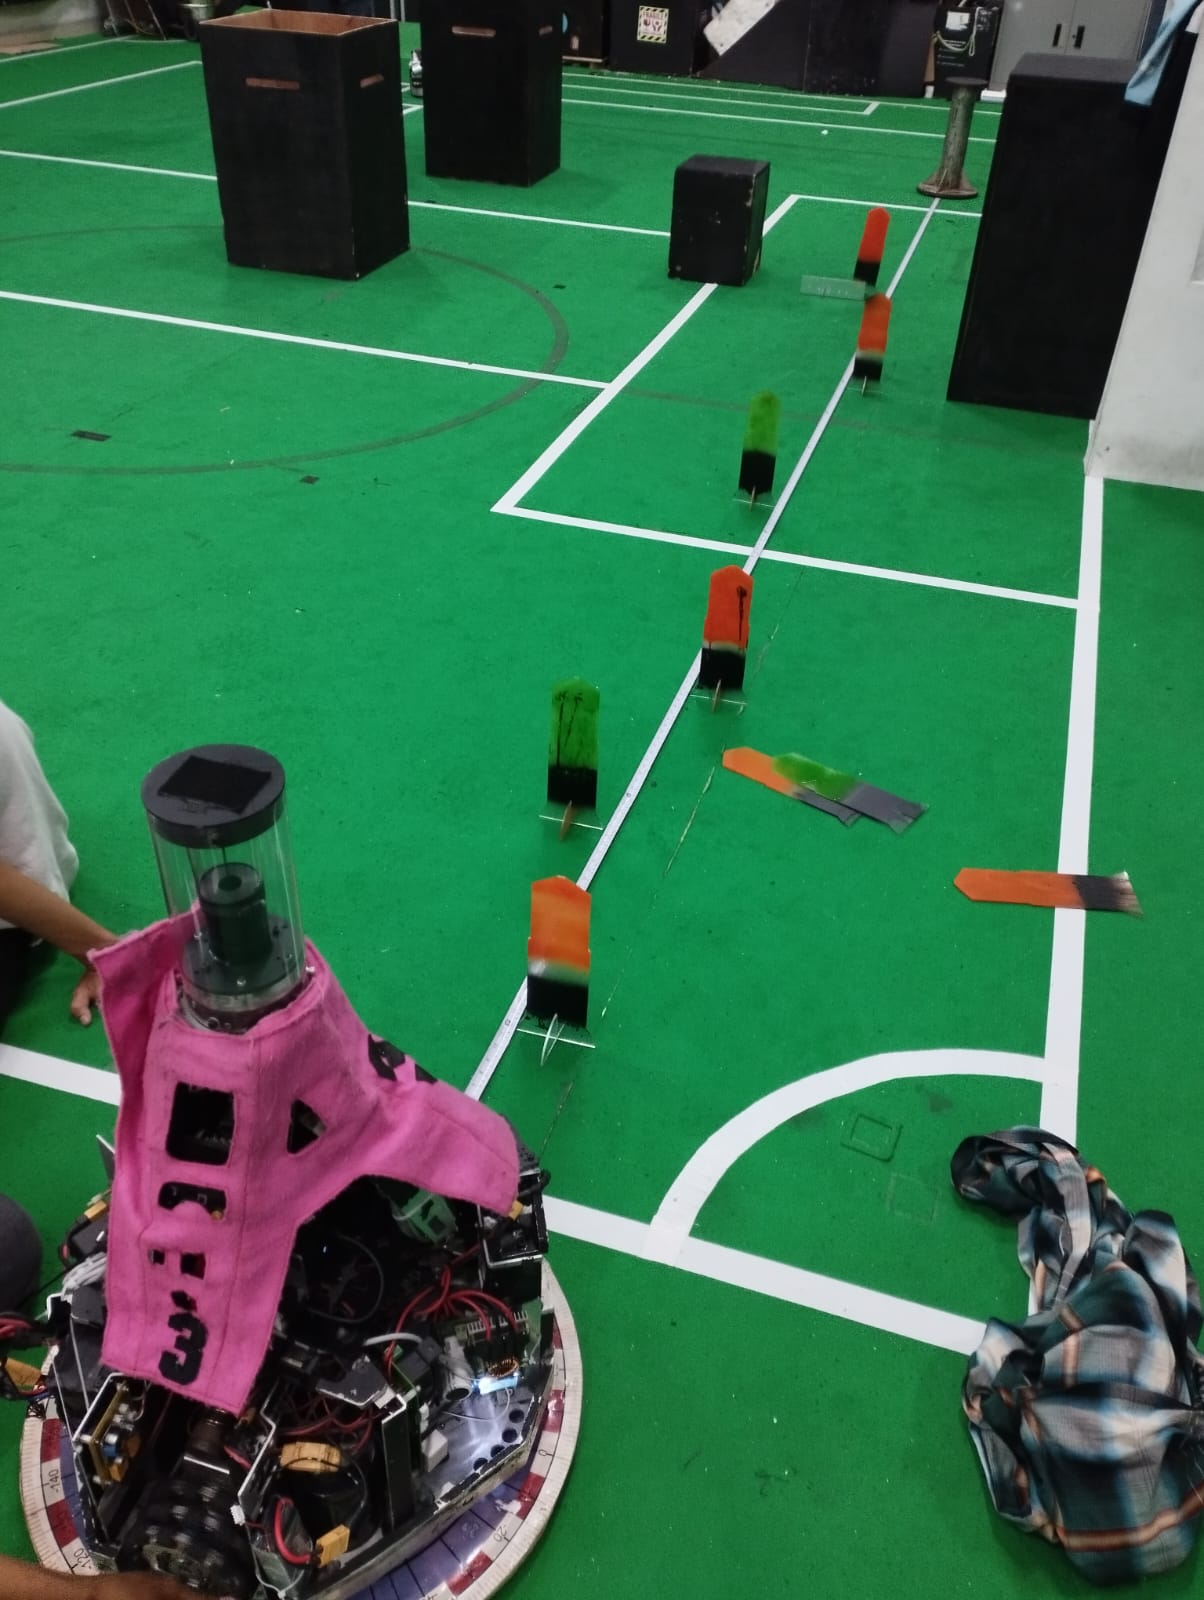
\includegraphics[scale=0.20]{gambar/ambil_data.jpeg}
  \caption{Persiapan robot.}
  \label{fig:persiapanrobot}
\end{figure}

Dikarenakan robot tidak memiliki display, maka untuk mengakses kamera perlu dilakukan dengan mengakses melalui program web yang telah disediakan oleh robot. Berikut adalah program robot untuk mengakses kamera dan mengirim ke web mengunakan \textit{websocket}.

\lstinputlisting[
  language=C++,
  caption={Program akses kamera.},
  label={lst:akseskamera}
]{program/akses_kamera.cpp}

\lstinputlisting[
  language=C++,
  caption={Program publish kamera.},
  label={lst:publishkamera}
]{program/publish_kamera.cpp}

\lstinputlisting[
  language=JavaScript,
  caption={Program akses kamera melalu web.},
  label={lst:kameraweb}
]{program/kamera_web.js}

\begin{figure}[H]
  \centering
  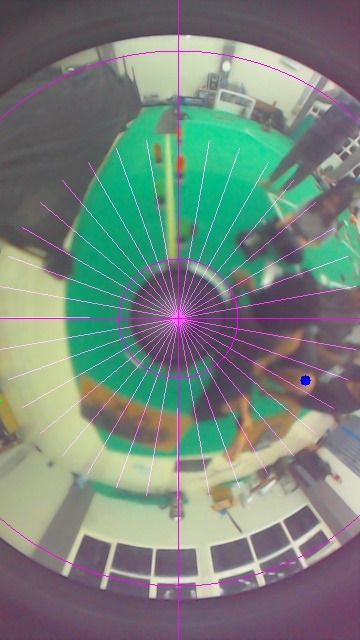
\includegraphics[scale=0.8]{gambar/iris_web.jpeg}
  \caption{Tampilan website robot.}
  \label{fig:webrobot}
\end{figure}

Dari tampilan website tersebut, warna merah pada lapangan bisa diklik dan akan muncul koordinat polar pada kamera. Lalu koordinat-koordinat tersebut akan disimpan ke dalam file. Adapun data yang diambil adalah sebagai berikut:
\begin{figure}[H]
  \centering
  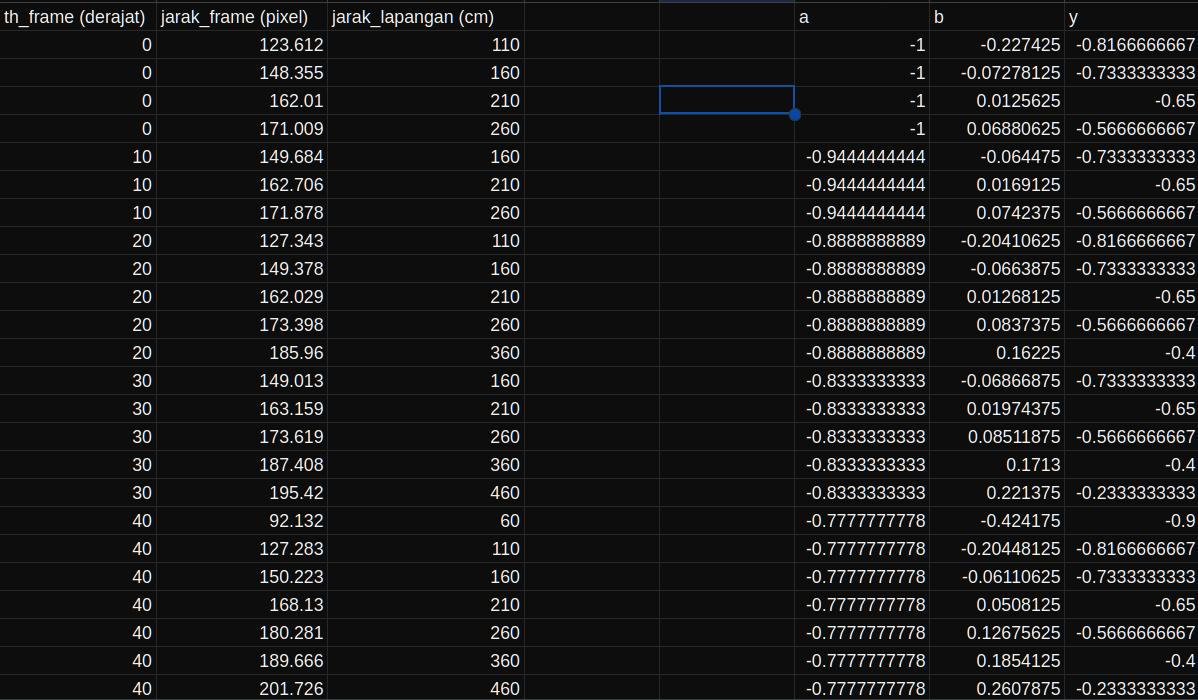
\includegraphics[scale=0.50]{gambar/data.jpg}
  \caption{Data \textit{training}.}
  \label{fig:datatraining}
\end{figure}

\section{\textit{Training} data
  \label{sec:trainingdata}}

Data yang telah diambil kemudian diolah dengan menggunakan program \textit{training} data. Program ini menggunakan metode \textit{Neural Network} untuk mengolah data tersebut. Berikut adalah program \textit{training} data. 

Adapun arsitektur \textit{Neural Network} yang digunakan adalah memiliki 2 \textit{hidden layer} dengan masing-masing 36 dan 36 \textit{neuron}. \textit{Activation function} yang digunakan adalah \textit{Sigmoid} dengan rumusan sebagai berikut: 

\begin{equation}
  \begin{aligned}
    f(x) &= \frac{1}{1 + e^{-x}}
  \end{aligned}
\end{equation}

Keuntungan menggunakan \textit{Sigmoid} adalah karena \textit{Sigmoid} memiliki rentang nilai antara 0 dan 1 yang sesuai dengan data yang akan diolah. 

\textit{Loss function} yang digunakan adalah \textit{Mean Squared Error} dengan rumusan sebagai berikut: 

\begin{equation}
  \begin{aligned}
    L(y, \hat{y}) &= \frac{1}{n} \sum_{i=1}^{n} (y_i - \hat{y_i})^2
  \end{aligned}
\end{equation}

\textit{Optimizer} yang digunakan adalah \textit{Adam} dengan \textit{learning rate} sebesar 0.0001.

Adapun epoch yang digunakan adalah sebanyak 300000 kali. Hal itu bisa berubah tergantung keadaan data yang di-\textit{train}. 

Adapun Arsitektur penuh dari \textit{Neural Network} yang digunakan adalah sebagai berikut: 

\begin{itemize}
    \item \( \mathbf{x} \in \mathbb{R}^2 \): Input data
    \item \( \mathbf{W}^{(1)} \in \mathbb{R}^{36 \times 2} \): weight layer pertama
    \item \( \mathbf{b}^{(1)} \in \mathbb{R}^{36} \): bias layer pertama
    \item \( \mathbf{W}^{(2)} \in \mathbb{R}^{36 \times 36} \): weight layer kedua
    \item \( \mathbf{b}^{(2)} \in \mathbb{R}^{36} \): bias layer kedua
    \item \( \mathbf{W}^{(3)} \in \mathbb{R}^{1 \times 36} \): weight layer ketiga
    \item \( \mathbf{b}^{(3)} \in \mathbb{R}^{1} \): bias layer ketiga
    \item \( \sigma \): sigmoid activation function
\end{itemize}

\begin{equation}
  \textbf{Input ke Hidden Layer Pertama}:
  \begin{aligned}
    \mathbf{z}^{(1)} &= \mathbf{W}^{(1)} \mathbf{x} + \mathbf{b}^{(1)} \\
    \mathbf{a}^{(1)} &= \sigma(\mathbf{z}^{(1)})
  \end{aligned}
\end{equation}

\begin{equation}
  \textbf{Hidden Layer Pertama ke Hidden Layer Kedua}:
  \begin{aligned}
    \mathbf{z}^{(2)} &= \mathbf{W}^{(2)} \mathbf{a}^{(1)} + \mathbf{b}^{(2)} \\
    \mathbf{a}^{(2)} &= \sigma(\mathbf{z}^{(2)})
  \end{aligned}
\end{equation}

\begin{equation}
  \textbf{Hidden Layer Kedua ke Output Layer}:
  \begin{aligned}
    \mathbf{z}^{(3)} &= \mathbf{W}^{(3)} \mathbf{a}^{(2)} + \mathbf{b}^{(3)} \\
    \mathbf{a}^{(3)} &= \mathbf{z}^{(3)}
  \end{aligned}
\end{equation}

% Contoh input potongan kode dari file
\lstinputlisting[
  language=Python,
  caption={Program \textit{train} data.},
  label={lst:traindata}
]{program/train.py}

\section{Pembuatan \textit{Lookup Table}
  \label{sec:pembuatanlut}}

Setelah data di-\textit{train} maka data tersebut akan dijadikan \textit{Lookup Table}. \textit{Lookup Table} ini berisi data-data yang telah di-\textit{train} sebelumnya. Berikut adalah rumusan untuk membuat \textit{Lookup Table} 2 dimensi: 

\begin{equation}
  \begin{aligned}
    size &= \theta\_max \times r\_max \\
    index &= \theta \times r\_max + r
  \end{aligned}
\end{equation}

Dari rumusan tersebut bisa didapat ukuran dari \textit{Lookup Table} yang akan dibuat dan index dari data yang akan dimasukkan ke dalam \textit{Lookup Table}.
Kemudian untuk nilai dari \textit{Lookup Table} itu sendiri berasal dari rumusan \textbf{3.4 - 3.6}.
Adapun program pembuatan \textit{Lookup Table} adalah sebagai berikut.

\lstinputlisting[
  language=Python,
  caption={Program pembuatan \textit{Lookup Table}.},
  label={lst:pembuatanlut}
]{program/save_lut.py}

\section{Pembacaan \textit{Lookup Table}
  \label{sec:pembacaanlut}}

Setelah \textit{Lookup Table} dibuat maka yang terakhir adalah membaca data dari \textit{Lookup Table} dengan rumusan sebagai berikut.  

\begin{equation}
  \begin{aligned}
    index &= \theta\_cam \times r\_max + r\_cam \\
    r\_real &= \textit{Lookup\_Table}[index] \\
    \theta\_real &= \theta\_cam
  \end{aligned}
\end{equation}

Proses tersebut dilakukan pada robot. Berikut adalah program pembacaan \textit{Lookup Table}.

\lstinputlisting[
  language=C++,
  caption={Program membaca \textit{Lookup Table}.},
  label={lst:membacalut}
]{program/read_lut.cpp} 
